\documentclass[12pt, a4paper]{scrreprt}

\renewcommand*\familydefault{\sfdefault} 
%\usepackage[T1]{fontenc}

\usepackage[english]{babel}
%\usepackage{cite}
\usepackage[utf8]{inputenc}
%\usepackage[onehalfspacing]{setspace}
\usepackage{geometry, textcomp}
\newgeometry{right=2cm,left=4cm, top=2.5cm, bottom=2.3cm, footnotesep=0.5cm}
%\usepackage[acronym]{glossaries}

\usepackage[printonlyused]{acronym}  % Abkürzungsverzeichnis [nur verwendete Abkürzugen]

%\glsenablehyper

%\makeglossaries

\usepackage{savesym}
\usepackage{amsmath,amssymb,amstext}
%\usepackage{graphics}
\savesymbol{iint}
\usepackage{txfonts}

\restoresymbol{TXF}{iint}
\usepackage[automark,headsepline,ilines,komastyle]{scrpage2}
\usepackage{blindtext}
\usepackage[euler]{textgreek}
\setlength{\parindent}{0pt}
\setlength{\headheight}{1.5\baselineskip}
\renewcommand{\baselinestretch}{1.5}

\pagestyle{scrheadings}
\clearscrheadfoot
\ihead[]{}
\chead[]{}
\ohead[]{\headmark \hfill \thepage}
\ifoot[]{}
\cfoot[]{}
\ofoot[]{}

\setheadsepline[\textwidth]{1pt}
\usepackage{tabularx}
\usepackage{colortbl}
\usepackage{multirow}
\usepackage{hhline}
\usepackage{array}
\usepackage{tocloft}
\usepackage[hidelinks]{hyperref}
\tocloftpagestyle{scrheadings}
\renewcommand{\chapterpagestyle}{scrheadings}
\usepackage[font=footnotesize]{caption}

\usepackage{tikz}
\usepackage{rotating} 

\newenvironment{packed_item}
	{\begin{itemize}
			\setlength{\itemsep}{0pt}
			\setlength{\topsep}{0pt}
			\setlength{\parsep}{0pt}
			\setlength{\parskip}{0pt}}
		{\end{itemize}}
	
\usepackage[style=authoryear, natbib=true, backend=biber]{biblatex}

\renewcommand{\nameyeardelim}{ }
\usepackage[babel,german=guillemets]{csquotes}

\makeatletter

\newrobustcmd*{\parentexttrack}[1]{%
	\begingroup
	\blx@blxinit
	\blx@setsfcodes
	\blx@bibopenparen#1\blx@bibcloseparen
	\endgroup}

\AtEveryCite{%
	\let\parentext=\parentexttrack%
	\let\bibopenparen=\bibopenbracket%
	\let\bibcloseparen=\bibclosebracket}

\makeatother

\usepackage{pstricks}
\usepackage{pstricks-add}

\bibliography{Lit.bib}

\usepackage[final]{pdfpages}

\begin{document}
%		\begin{titlepage}
			\begin{center}
			%\setlength{\headheight}{1.5\baselineskip}
			\renewcommand{\baselinestretch}{1.5}
					\textbf{\large FOM - Hochschule für Oekonomie \& Management \\
						Hamburg \\
						\ \\
						Master-Studiengang Big Data \& Business Analytics \\
						3. Semester \\
						\ \\
						Development of a system to control and monitor blood pressure \ \\
						measurements to prevent cardiovascular disease \ \\
						\ \\
						}
						
					\textrm{
						\ \\
						Betreuer: Prof. Dr. Kai Brüssau \\
						\ \\
						Autor: Jacqueline Franßen \\
						\ \\
						Matrikel-Nr: 496804 \\
						\ \\
						3. Fachsemester \\
						\ \\
						Hamburg, den 29.02.2020 \\
						}
			\end{center}
		\end{titlepage}

%\includepdf{Image/Deckblatt.pdf}

			\setcounter{tocdepth}{3}
			\setcounter{secnumdepth}{3}		
			\pagenumbering{Roman}
			\thispagestyle{empty}
			\pdfbookmark{\contentsname}{toc}\tableofcontents
			\newpage
			\listoffigures
			\listoftables

			\pagenumbering{arabic}
			\thispagestyle{empty}
\chapter{Abstract}\label{abstract}

only documentation of blood pressure values, not measurement (current hardware of smartphone not able)

\chapter{Introduction}\label{introduction}

\section{Problem statement}


\section{Aim and scope of this work}

%describe aim
The first aim of this scientific work is to develop a solution ...
%describe scope
What is important, the developed model is only a reference model....

\chapter{Fundamentals}\label{fundamentals}

\section{Related Work}

Deep learning methods use multiple layers of nonlinear processing units for feature extraction and transformation and to find deep relationships between complex variations under supervised and unsupervised procedures.

\subsection{\ac{iarc}}

The \ac{iarc} is a association with the aim to raise the development within cancer treatment and research. It was formed by the \ac{who} and has its main location in France. Besides, it provides a large library of cancerogens for users.



\section{Analysis and Development}

\subsection{Design Thinking Methods}



\subsection{Vertical latter}

In the given figure, a vertical letter shows the initially planned goals and features of the app. The X-Axis shows the time steps whereas the Y-Axis explains the complexity of tasks. The higher on task is mentioned, the more complex it is to realize.



\subsection{How might we?}


\subsection{Stakeholder Map}

Figure gives an overview of potential stakeholders. As can be seen in this figure, there are four groups of users: patients, doctors, the IT appartment of the hospital and the 



\subsection{Empathy Map}

In this section, three primary developed persona were developed. They should represent each of them a specific user of the user groups. Figures  give an overview of what each persona feels and thinks about the treatment process of cancer, especially skin cancer. Moreover, the empathy maps were developed before asking affected patients and might differ from real opinions. But during the first step of this project this method serves well to specify the business case. 




\subsection{Hills}

The design thinking method "hills" is a special method to prioritize the real needs of users and to set special goals that differ the solution from existing apps. The second fact is really important for development. As this method answers the three questions 'WHO', 'WHAT' and 'HOW', the focus is on the most important feature which shall be realized. In further planning, this feature can be divided into multiple 'todos'  during development process. This raises the practicability of the product and accelerates the development. Figure shows the developed hills which explain two different point of views: On the one hand, patient's view and on the otherhand, the doctor's view.
To give an example, one hill is expressed as: 'As a patient, i would like to have a reliable, real-time and easy-to-understand diagnose about my type of skin cancer.'
Another hill is: 'As a doctor, i would like the application to outline potential skin tumors and to calculate the  approximate amount of medication and how it has to be administered. Furthermore, there should be a check whether the medication is available at the hospital's pharmacy or not. If the medication is not available, it should be ordered immediately and delivered to the patient.


\subsection{User Journey}



\section{User Research}
\subsection{User interviews}
\subsection{What is important? - Relevant features}
\subsection{How can processes be improved?}


\section{Development of system to predict metastasis and recidives} 

\subsection{Challenges of development}


\subsection{Data Research}
\paragraph{Kaggle dataset}


\subsection{\ac{crisp-dm}: Model Planning and Learning}

\subsection{U-net architecture to for medical imaging}



\subsection{Testing}
\subsection{Results} 

\chapter{Results}
\section{Validation of results}
\section{Limitation in the development process}

\chapter{Conclusion and Outlook}
\section{Conclusion}
\section{Outlook}


\chapter{Abbreviations}
\begin{acronym}[CRISP-DM]
\acro{crisp-dm}[CRISP-DM]{CRoss-Industry Standard Process for Data Mining}
\acro{cfo}[CFO]{Chief Financial Officer}
\acro{who}[WHO]{World Health Organization}
\acro{iarc}[IARC]{International Agency for Research on Cancer}
\acro{ham10000}[HAM10000]{Human Against Machine with 10000 training images}
\end{acronym}

\printbibliography[heading=bibintoc]

\chapter{Appendix A}\label{appendix a}
\ohead[]{Ehrenwörtliche Erklärung \hfill \thepage}

\null\vfill
\textbf{Ehrenwörtliche Erklärung}

Hiermit versichere ich, dass die vorliegende Arbeit von mir selbstständig und ohne unerlaubte Hilfe angefertigt worden ist, insbesondere dass ich alle Stellen, die wörtlich oder annähernd wörtlich aus Veröffentlichungen entnommen sind, durch Zitate als solche gekennzeichnet habe. Ich versichere auch, dass die von mir eingereichte schriftliche Version mit der digitalen Version übereinstimmt. Weiterhin erkläre ich, dass die Arbeit in gleicher oder ähnlicher Form noch keiner Prüfungsbehörde / Prüfungsstelle vorgelegen hat. Ich erkläre mich damit nicht einverstanden, dass die Arbeit der Öffentlichkeit zugänglich gemacht wird. Ich erkläre mich damit einverstanden, dass die Digitalversion dieser Arbeit zwecks Plagiatsprüfung auf die Server externer Anbieter hochgeladen werden darf. Die Plagiatsprüfung stellt keine Zurverfügungstellung für die Öffentlichkeit dar.

\ \\ \ \\ 


Ort, Datum (Vorname Nachname)

\vfill
%\chapter{Appendix B}\label{appendix b}
%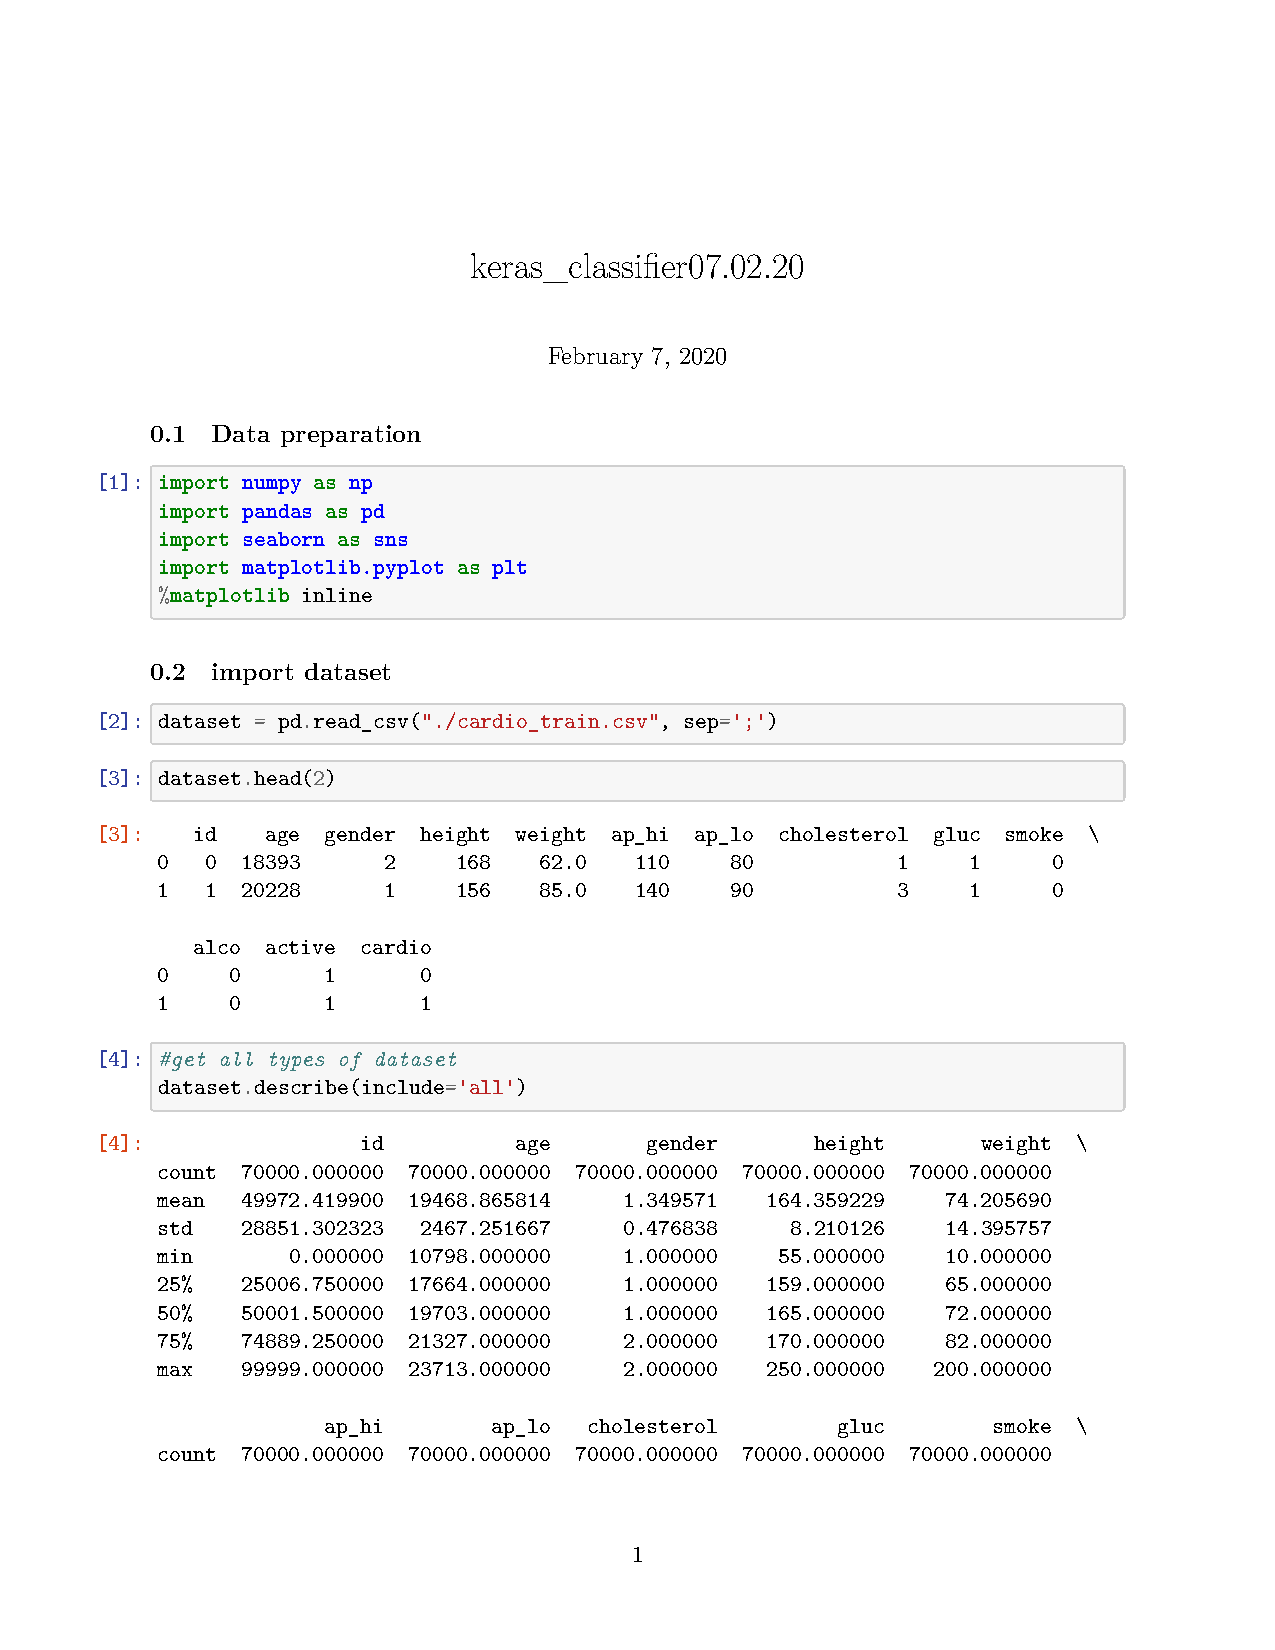
\includepdf[pages=-]{keras_classifier.pdf}

\end{document}
